\subsection{Sviluppatori}
\subsubsection{Panoramica sviluppatore}
\begin{figure}[H]
	\centering
	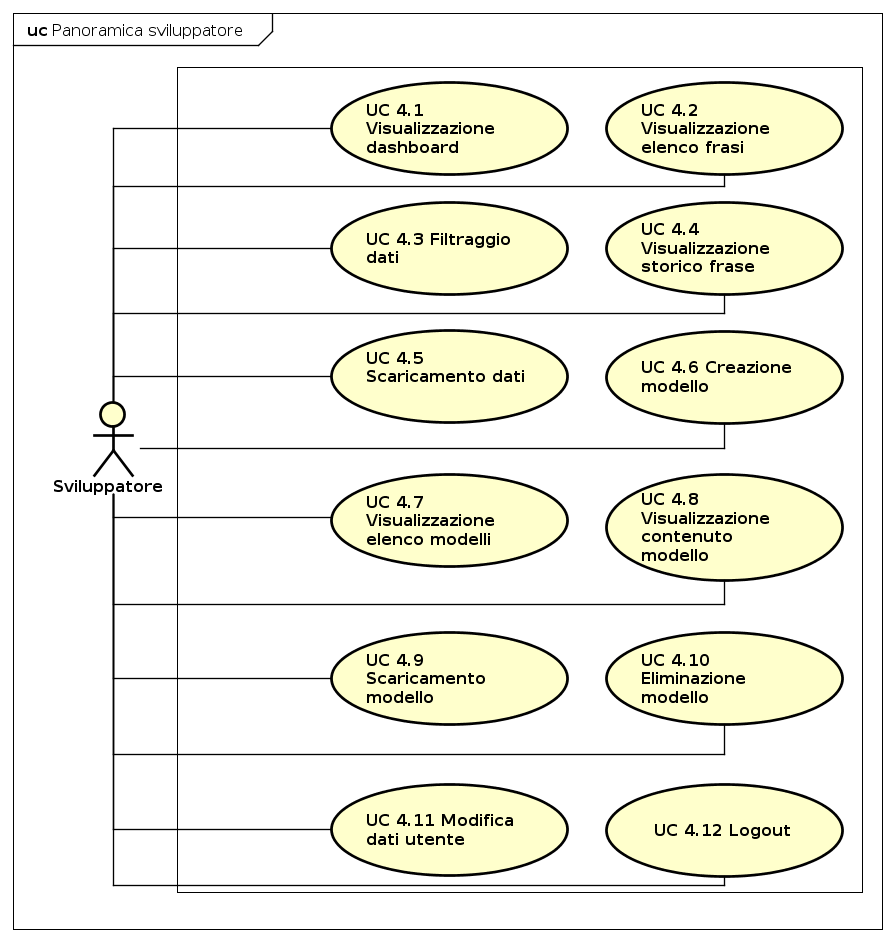
\includegraphics[width=17cm, keepaspectratio]{img/UC4x.png} 
	\caption{Panoramica sviluppatore}\label{fig:4x}
\end{figure}
\subsubsection{UC 4.1 - Visualizzazione dashboard}
\begin{itemize}
	\item[•]\textbf{Attori}: Sviluppatore;
	\item[•]\textbf{Descrizione}: lo sviluppatore ha effettuato l'autenticazione e visualizza la propria dashboard;
	\item[•]\textbf{Precondizione}: lo sviluppatore ha effettuato l'autenticazione;
	\item[•]\textbf{Postcondizione}: lo sviluppatore visualizza la propria dashboard; 
	\item[•]\textbf{Flusso degli eventi}: lo sviluppatore ha effettuato l'autenticazione e viene automaticamente reindirizzato alla pagina che contiene la dashboard.
\end{itemize}
\subsubsection{UC 4.2 - Visualizzazione elenco frasi}
\begin{itemize}
	\item[•]\textbf{Attori}: Sviluppatore;
	\item[•]\textbf{Descrizione}: lo sviluppatore visualizza un elenco di frasi accompagnate 
	dalla data di creazione e dall’autore ordinate cronologicamente;
	\item[•]\textbf{Precondizione}:  lo sviluppatore si è autenticato nel sistema e visualizza la propria dashboard.
	\item[•]\textbf{Postcondizione}: lo sviluppatore visualizza l'elenco delle preposizioni ordinate cronologicamente comprensive di analisi grammaticale, data, autore e livello di attendibilità;
	\item[•]\textbf{Flusso degli eventi}: lo sviluppatore ha selezionato la voce relativa alla pagina contenente l’elenco delle frasi e ne visualizza il contenuto. 
\end{itemize}
\subsubsection{UC 4.3 - Filtraggio dei dati}
\begin{figure}[H]
	\centering
	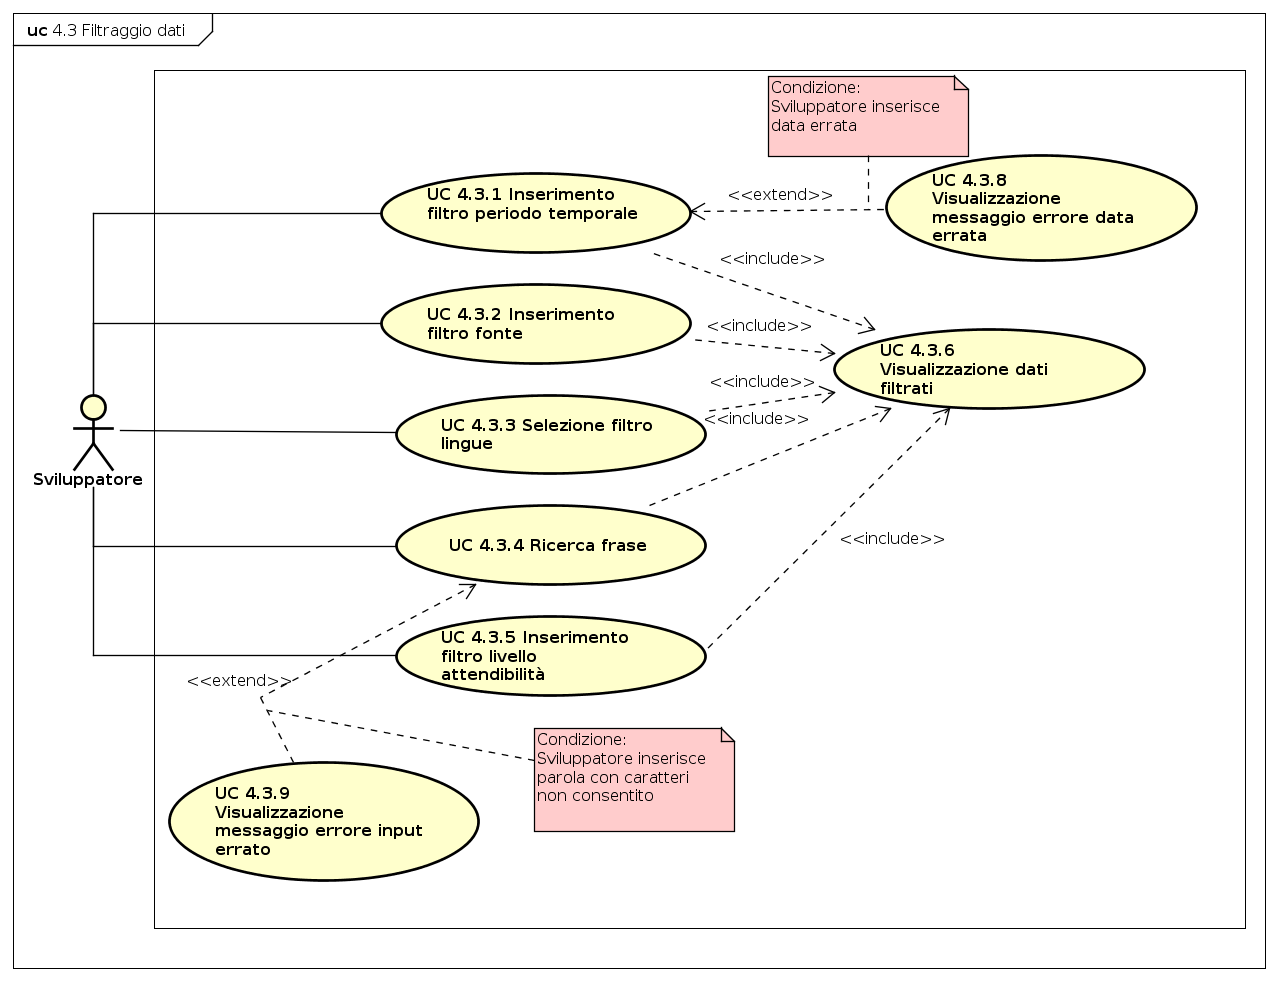
\includegraphics[width=14cm, keepaspectratio]{img/UC430.png} 
	\caption{Caso d'uso UC 4.3}\label{fig:430}
\end{figure}
\begin{itemize}
	\item[•]\textbf{Attori}: Sviluppatore;
	\item[•]\textbf{Descrizione}: lo sviluppatore applica dei filtri ai dati, ottenendo solo quelli d'interesse;
	\item[•]\textbf{Precondizione}: lo sviluppatore visualizza le proposizioni in ordine cronologico (UC 4.2);
	\item[•]\textbf{Postcondizione}: lo sviluppatore visualizza i dati che rispettano i filtri scelti;
	\item[•]\textbf{Flusso degli eventi}:
	\begin{enumerate}
		\item UC 4.3.1 - Inserimento filtro periodo temporale;
		\item UC 4.3.2 - Inserimento filtro {fonte}\ped{G};
		\item UC 4.3.3 - Selezione filtro lingue;
		\item UC 4.3.4 - Ricerca parole chiave;
		\item UC 4.3.5 - Inserimento filtro livello attendibilità.
	\end{enumerate}
	\item[•]\textbf{Estensioni}:
	\begin{enumerate}
		\item UC 4.3.7 - Rimozione filtro;
		\item UC 4.3.8 - Visualizzazione messaggio errore data errata;
		\item UC 4.3.9 - Visualizzazione messaggio errore input errato.
	\end{enumerate}
	\item[•]\textbf{Inclusioni}:
	\begin{enumerate}
		\item UC 4.3.6 - Visualizzazione dati filtrati.
	\end{enumerate}
\end{itemize}
\subsubsection{UC 4.3.1 - Inserimento filtro periodo temporale}
\begin{itemize}
	\item[•]\textbf{Attori}: Sviluppatore;
	\item[•]\textbf{Descrizione}: lo sviluppatore seleziona un periodo temporale, ottenendo i dati salvati in un determinato arco di tempo;
	\item[•]\textbf{Precondizione}: lo sviluppatore visualizza le proposizioni in base ai filtri stabiliti;
	\item[•]\textbf{Postcondizione}: lo sviluppatore visualizza le frasi che rispettano il periodo di tempo indicato nel filtro;
	\item[•]\textbf{Flusso degli eventi}: 
	\begin{enumerate}
		\item Scelta data inizio periodo;
		\item Scelta data fine periodo.
	\end{enumerate}
	\item[•]\textbf{Estensioni}: 
	\begin{enumerate}
		\item UC 4.3.7 - Rimozione filtro;
		\item UC 4.3.8 - Visualizzazione messaggio errore data errata;
	\end{enumerate}
	\item[•]\textbf{Inclusioni}:
	\begin{enumerate}
		\item UC 4.3.6 - Visualizzazione dati filtrati.
	\end{enumerate}
\end{itemize}

\subsubsection{UC 4.3.2 - Inserimento filtro fonte}
\begin{itemize}
	\item[•]\textbf{Attori}: Sviluppatore;
	\item[•]\textbf{Descrizione}: lo sviluppatore seleziona una o più fonti degli esercizi, come ad esempio le correzione provenienti da determinati docenti o dal sistema di correzione automatico;
	\item[•]\textbf{Precondizione}: lo sviluppatore visualizza le proposizioni in base ai filtri stabiliti;
	\item[•]\textbf{Postcondizione}: lo sviluppatore ha impostato i valori del filtro fonte, pertanto vuole visualizzare tutte le proposizioni inserite da una determinata fonte ed eventualmente gli altri filtri;
	\item[•]\textbf{Flusso degli eventi}: lo sviluppatore seleziona da un elenco le fonti di cui è interessato visualizzare i dati;
	\item[•]\textbf{Estensioni}: 
	\begin{enumerate}
		\item UC 4.3.7 - Rimozione filtro.
	\end{enumerate}
	\item[•]\textbf{Inclusioni}:
	\begin{enumerate}
		\item UC 4.3.6 - Visualizzazione dati filtrati.
	\end{enumerate}
\end{itemize}

\subsubsection{UC 4.3.3 -  Selezione filtro lingue}
\begin{itemize}
	\item[•]\textbf{Attori}: Sviluppatore;
	\item[•]\textbf{Descrizione}: lo sviluppatore seleziona una o più lingue da un elenco di lingue predefinito al fine di ottenere solamente le proposizioni scritte in tali lingue;
	\item[•]\textbf{Precondizione}: lo sviluppatore visualizza le proposizioni in base ai filtri stabiliti;
	\item[•]\textbf{Postcondizione}: lo sviluppatore ha stabilito i valori di filtraggio relativi alle lingue, quindi visualizza tutte le frasi scritte in tale lingua e che soddisfano anche gli altri filtri applicati;
	\item[•]\textbf{Flusso degli eventi}: lo sviluppatore seleziona da un elenco le lingue di cui è interessato vedere le proposizioni memorizzate;
	\item[•]\textbf{Estensioni}: 
	\begin{enumerate}
		\item UC 4.3.7 - Rimozione filtro.
	\end{enumerate}
	\item[•]\textbf{Inclusioni}:
	\begin{enumerate}
		\item UC 4.3.6 - Visualizzazione dati filtrati.
	\end{enumerate}
\end{itemize}

\subsubsection{UC 4.3.4 - Ricerca frase}
\begin{itemize}
	\item[•]\textbf{Attori}: Sviluppatore;
	\item[•]\textbf{Descrizione}: lo sviluppatore scrive una o più parole chiave al fine di cernere le frasi contenenti tali parole;
	\item[•]\textbf{Precondizione}: lo sviluppatore visualizza le frasi in base al filtraggio scelto;
	\item[•]\textbf{Postcondizione}: lo sviluppatore ha impostato le parole chiave e visualizza solamente le frasi che contengono solamente quelle parole e che rispettano gli altri filtri inseriti;
	\item[•]\textbf{Flusso degli eventi}: lo sviluppatore inserisce una stringa rappresentate una o più parole chiave che devono essere contenute nelle stringhe che intende visualizzare;
	\item[•]\textbf{Estensioni}: 
	\begin{enumerate}
		\item UC 4.3.7 - Rimozione filtro;
		\item UC 4.3.9 - Visualizzazione messaggio di errore input errato.
	\end{enumerate}
	\item[•]\textbf{Inclusioni}:
	\begin{enumerate}
		\item UC 4.3.6 - Visualizzazione dati filtrati.
	\end{enumerate}
\end{itemize}

\subsubsection{UC 4.3.5 - Inserimento filtro livello attendibilità}
\begin{itemize}
	\item[•]\textbf{Attori}: Sviluppatore;
	\item[•]\textbf{Descrizione}: lo sviluppatore seleziona un valore numerico rappresentante il livello di attendibilità delle frasi che vuole visualizzare, ovvero frasi le cui correzioni sono uguali a quelle di altre insegnanti acquisiscono un livello di attendibilità maggiore rispetto ad altre;
	\item[•]\textbf{Precondizione}: i valori di uno o più filtri sono stati inseriti;
	\item[•]\textbf{Postcondizione}: lo sviluppatore ha selezionato il livello di attendibilità e visualizza solamente le frasi che hanno tale livello di attendibilità, cioè che hanno ricevuto la stessa correzione da più insegnanti, e che rispettano eventualmente gli altri filtri inseriti.
	\item[•]\textbf{Flusso degli eventi}: lo sviluppatore seleziona da un elenco predefinito il livello di attendibilità desiderato.
\item[•]\textbf{Estensioni}: 
	\begin{enumerate}
		\item UC 4.3.7 - Rimozione filtro.
	\end{enumerate}
	\item[•]\textbf{Inclusioni}:
	\begin{enumerate}
		\item UC 4.3.6 - Visualizzazione dati filtrati.
	\end{enumerate}
\end{itemize}



\subsubsection{UC 4.3.6 - Visualizzazione dati filtrati}
\begin{itemize}
	\item[•]\textbf{Attori}: Sviluppatore;
	\item[•]\textbf{Descrizione}: selezionato uno o più filtri, i dati vengono mostrati secondo i vincoli inseriti;
	\item[•]\textbf{Precondizione}: i valori di uno o più filtri sono stati inseriti;
	\item[•]\textbf{Postcondizione}: lo sviluppatore visualizza solamente le preposizioni che rispettano i filtri inseriti.
	\item[•]\textbf{Flusso degli eventi}: lo sviluppatore inserisce un filtro e visualizza tutti i dati che rispettano tale filtro.
\end{itemize}

\subsubsection{UC 4.3.7 - Rimozione filtro}
\begin{itemize}
	\begin{figure}[H]
		\centering
		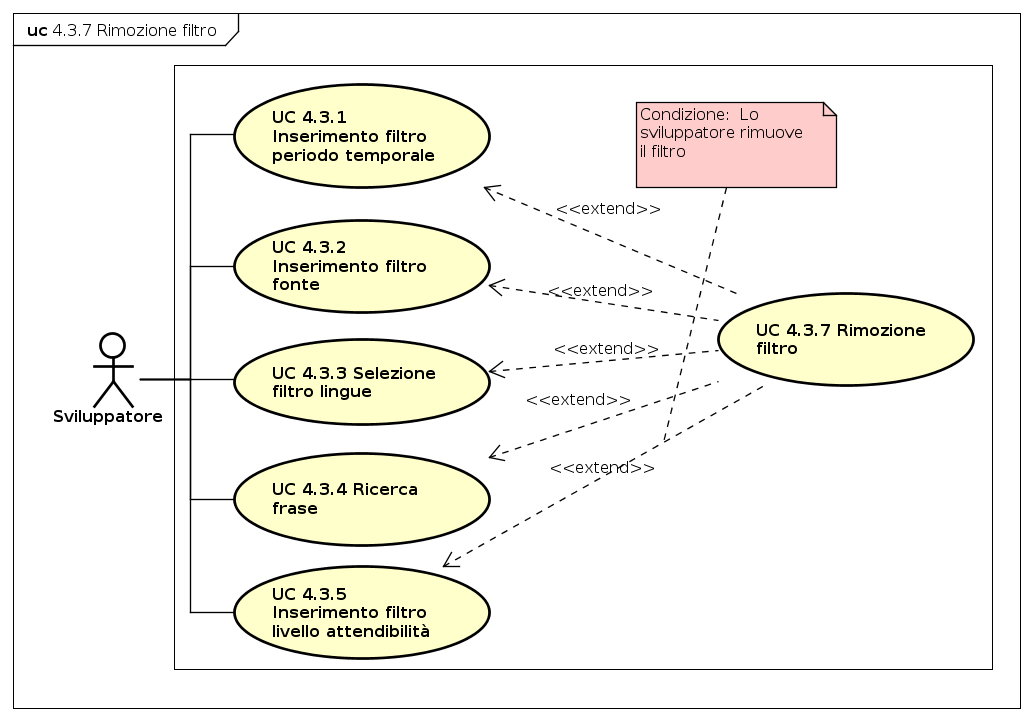
\includegraphics[width=14cm, keepaspectratio]{img/UC437.png} 
		\caption{Caso d'uso UC 4.3.7 relativo alla rimozione dei filtri.}\label{fig:437}
	\end{figure}
	\item[•]\textbf{Attori}: Sviluppatore;
	\item[•]\textbf{Descrizione}: lo sviluppatore cancella il valore del filtro selezionato.
	\item[•]\textbf{Precondizione}: il filtro contiene un valore ed è applicato un filtraggio ai dati rispettando le condizioni di tale filtro;
	\item[•]\textbf{Postcondizione}: il filtro è stato rimosso pertanto i dati visualizzati non rispetteranno più tale vincolo;
	\item[•]\textbf{Flusso degli eventi}: lo sviluppatore seleziona il filtro e lo rimuove.
\end{itemize}

\subsubsection{UC 4.3.8 - Visualizzazione messaggio errore data errata}
\begin{itemize}
	\item[•]\textbf{Attori}: Sviluppatore;
	\item[•]\textbf{Descrizione}: lo sviluppatore visualizza un messaggio di errore sul periodo selezionato;
	\item[•]\textbf{Precondizione}: lo sviluppatore ha inserito una data non conforme all'interno del filtro relativo al periodo temporale;
	\item[•]\textbf{Postcondizione}: il filtro è stato erroneamente inserito pertanto viene visualizzato un messaggio di errore;
	\item[•]\textbf{Flusso degli eventi}: lo sviluppatore ha inserito una data non conforme, cioè che non rispetta il formato stabilito o che indica un periodo temporale non idoneo, pertanto visualizza un messaggio di errore.
\end{itemize}

\subsubsection{UC 4.3.9 - Visualizzazione messaggio errore input errato}
\begin{itemize}
	\item[•]\textbf{Attori}: Sviluppatore;
	\item[•]\textbf{Descrizione}: lo sviluppatore visualizza un messaggio di errore sulla ricerca.
	\item[•]\textbf{Precondizione}: lo sviluppatore ha inserito una frase non conforme;
	\item[•]\textbf{Postcondizione}: lo sviluppatore visualizza un messaggio di errore relativo 
	all'inserimento di un input errato, cioè non conforme a ciò che il sistema si attendeva.
	\item[•]\textbf{Flusso degli eventi}: lo sviluppatore inserisce un input non conforme, cioè contenente caratteri non ammessi, e visualizza un messaggio di input errato.
\end{itemize}

\subsubsection{UC 4.4 - Visualizzazione storico frase}
\begin{itemize}
	\item[•]\textbf{Attori}: Sviluppatore;
	\item[•]\textbf{Descrizione}: lo sviluppatore seleziona una frase dall'elenco e ne visualizza lo storico contenente la correzione fornita dal sistema automatico, ed eventualmente quelle redatte anche da insegnanti diversi;
	\item[•]\textbf{Precondizione}: lo sviluppatore visualizza le frasi in base ai filtri stabiliti;
	\item[•]\textbf{Postcondizione}: lo sviluppatore visualizza tutte le correzioni della frase;
	\item[•]\textbf{Flusso degli eventi}: lo sviluppatore seleziona la frase e appare lo storico della frase.
\end{itemize}

\subsubsection{UC 4.5 - Scaricamento dati}
\begin{figure}[H]
	\centering
	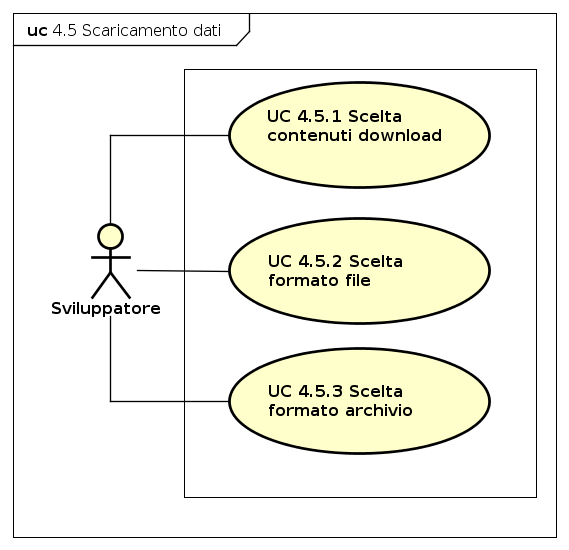
\includegraphics[width=10cm, keepaspectratio]{img/UC450.png} 
	\caption{Caso d'uso UC 4.5}\label{fig:450}
\end{figure}
\begin{itemize}
	\item[•]\textbf{Attori}: Sviluppatore;
	\item[•]\textbf{Descrizione}: lo sviluppatore esegue il download dei dati d'interesse;
	\item[•]\textbf{Precondizione}: lo sviluppatore visualizza i dati in ordine cronologico, e nel caso siano applicati filtri, vede solo i dati che rispettano tali filtri;
	\item[•]\textbf{Postcondizione}: lo sviluppatore scarica un file contenente le analisi grammaticali in formato anonimo;
	\item[•]\textbf{Flusso degli eventi}:
	\begin{enumerate}
		\item UC 4.5.1 - Scelta contenuti download;
		\item UC 4.5.2 - Scelta formato file;
		\item UC 4.5.3 - Scelta formato archivio.
	\end{enumerate}
\end{itemize}

\subsubsection{UC 4.5.1 - Scelta contenuti download}
\begin{itemize}
	\item[•]\textbf{Attori}: Sviluppatore;
	\item[•]\textbf{Descrizione}: lo sviluppatore sceglie gli elementi di interesse che vuole siano scaricati una volta completata la procedura di download;
	\item[•]\textbf{Precondizione}: lo sviluppatore visualizza le preposizioni in base ai filtri stabiliti;
	\item[•]\textbf{Postcondizione}: lo sviluppatore visualizza i contenuti che intende scaricare, come ad esempio lo storico di una frase;
	\item[•]\textbf{Flusso degli eventi}: lo sviluppatore seleziona dall'elenco, eventualmente filtrato, le proposizioni d'interesse, come ad esempio quelle provenienti da i soli docenti selezionati.
\end{itemize}

\subsubsection{UC 4.5.2 - Scelta formato file}
\begin{itemize}
	\item[•]\textbf{Attori}: Sviluppatore;
	\item[•]\textbf{Descrizione}:  lo sviluppatore seleziona da un elenco prestabilito il formato dei file che intende scaricare;
	\item[•]\textbf{Precondizione}: lo sviluppatore non ha stabilito il formato dei file che intende scaricare;
	\item[•]\textbf{Postcondizione}: lo sviluppatore ha stabilito il formato dei file che intende scaricare;
	\item[•]\textbf{Flusso degli eventi principale}:  lo sviluppatore seleziona dall'elenco prestabilito un'opzione che determina il formato dei file che contengono i dati precedentemente scelti.
\end{itemize}

\subsubsection{UC 4.5.3 - Scelta formato archivio}
\begin{itemize}
	\item[•]\textbf{Attori}: Sviluppatore;
	\item[•]\textbf{Descrizione}: lo sviluppatore seleziona da un elenco prestabilito il formato dell'archivio compresso con cui vuole che i dati d'interesse siano compressi;
	\item[•]\textbf{Precondizione}: il formato dell'archivio contenente i dati d'interesse non è definito;
	\item[•]\textbf{Postcondizione}: il formato dell'archivio contenente i dati d'interesse è stato definito;
	\item[•]\textbf{Flusso degli eventi}: lo sviluppatore seleziona dall'elenco prestabilito un'opzione che determina il formato dell'archivio che contiene i file relativi ai dati precedentemente scelti.
\end{itemize}


\subsubsection{UC 4.6 - Creazione modello}
\begin{figure}[H]
	\centering
	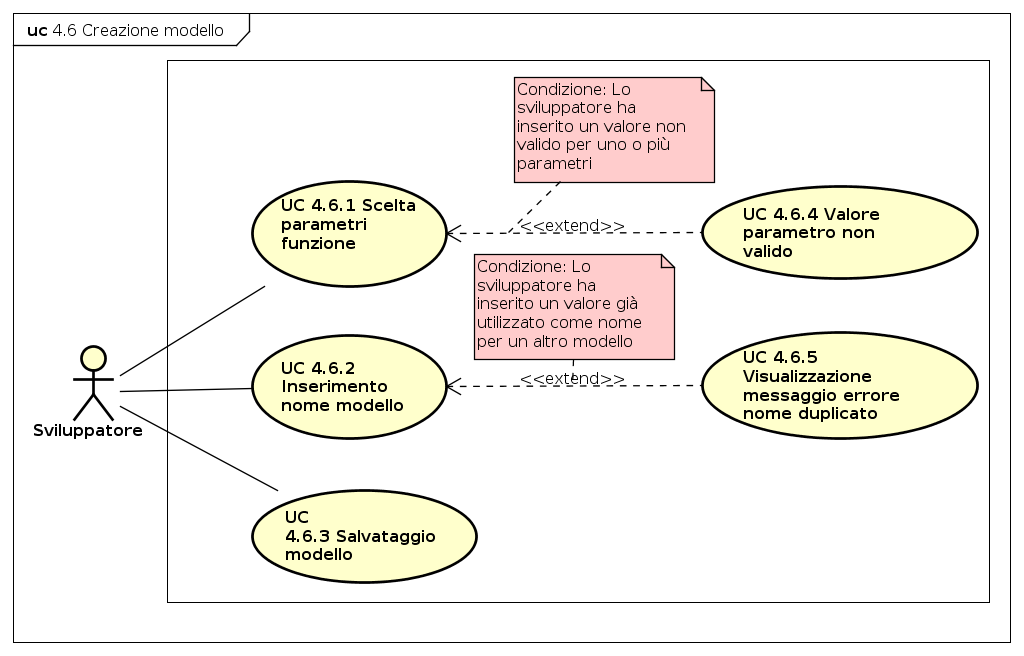
\includegraphics[width=17cm, keepaspectratio]{img/UC460.png} 
	\caption{Caso d'uso UC 4.6}\label{fig:460}
\end{figure}
\begin{itemize}
	\item[•]\textbf{Attori}: Sviluppatore;
	\item[•]\textbf{Descrizione}: lo sviluppatore crea un nuovo modello;
	\item[•]\textbf{Precondizione}: lo sviluppatore non ha creato il modello;
	\item[•]\textbf{Postcondizione}: lo sviluppatore ha creato un nuovo modello;
	\item[•]\textbf{Flusso degli eventi}:  
	\begin{enumerate}
		\item UC 4.6.1 - Scelta parametri funzione;
		\item UC 4.6.2 - Inserimento nome modello;
		\item UC 4.6.3 - Salvataggio modello.
	\end{enumerate}
	\item[•]\textbf{Estensioni}:  
	\begin{enumerate}
		\item UC 4.6.4 - Valore parametro non valido;
		\item UC 4.6.5 - Visualizzazione messaggio errore nome duplicato.
	\end{enumerate}
\end{itemize}

\subsubsection{UC 4.6.1 - Scelta parametri funzione}
\begin{itemize}
	\item[•]\textbf{Attori}: Sviluppatore;
	\item[•]\textbf{Descrizione}: lo sviluppatore sceglie i parametri della funzione per la creazione di un nuovo modello con i relativi valori associati;
	\item[•]\textbf{Precondizione}: lo sviluppatore non ha scelto i parametri da inserire;
	\item[•]\textbf{Postcondizione}: lo sviluppatore ha inserito i parametri per la creazione di un nuovo modello;
	\item[•]\textbf{Flusso degli eventi}:  lo sviluppatore inserisce tutti i parametri necessari che verranno impiegati nella realizzazione del modello.
	\item[•] \textbf{Estensioni}: 
	\begin{enumerate}
		\item UC 4.6.4 - Valore parametro non valido.
	\end{enumerate}
\end{itemize}

\subsubsection{UC 4.6.2 - Inserimento nome modello}
\begin{itemize}
	\item[•]\textbf{Attori}: Sviluppatore;
	\item[•]\textbf{Descrizione}: lo sviluppatore inserisce il nome per il modello che intende salvare;
	\item[•]\textbf{Precondizione}: lo sviluppatore non ha inserito il nome del modello;
	\item[•]\textbf{Postcondizione}: lo sviluppatore ha inserito il nome del modello;
	\item[•]\textbf{Flusso degli eventi}: lo sviluppatore inserisce una stringa che definisce il nome del modello che verrà memorizzato.
	\item[•] \textbf{Estensioni}: 
	\begin{enumerate}
		\item UC 4.5.5 - Visualizzazione messaggio errore nome duplicato.
	\end{enumerate}
\end{itemize}

\subsubsection{UC 4.6.3 - Salvataggio modello}
\begin{itemize}
	\item[•]\textbf{Attori}: Sviluppatore;
	\item[•]\textbf{Descrizione}: lo sviluppatore salva il modello di cui ha definito il nome;
	\item[•]\textbf{Precondizione}: lo sviluppatore ha inserito il nome del modello;
	\item[•]\textbf{Postcondizione}: lo sviluppatore ha salvato il modello;
	\item[•]\textbf{Flusso degli eventi}: lo sviluppatore seleziona l'opzione relativa al salvataggio che comporta il salvataggio del modello.
\end{itemize}

\subsubsection{UC 4.6.4 - Valore parametro non valido}
\begin{itemize}
	\item[•]\textbf{Attori}: Sviluppatore;
	\item[•]\textbf{Descrizione}: il sistema segnala un messaggio di errore relativo al valore del parametro non valido;
	\item[•]\textbf{Precondizione}: lo sviluppatore ha inserito il valore del parametro;
	\item[•]\textbf{Postcondizione}: lo sviluppatore visualizza un messaggio di errore relativo al valore del parametro non valido;
	\item[•]\textbf{Flusso degli eventi}:  lo sviluppatore ha inserito un valore per il parametro non valido pertanto visualizza un messaggio d'errore.
\end{itemize}
\subsubsection{UC 4.6.5 - Visualizzazione messaggio errore nome duplicato}
\begin{itemize}
	\item[•]\textbf{Attori}: Sviluppatore;
	\item[•]\textbf{Descrizione}: lo sviluppatore visualizza un messaggio di errore relativo all'inserimento di un modello avente lo stesso nome di uno già inserito;
	\item[•]\textbf{Precondizione}: lo sviluppatore ha inserito il nome del modello;
	\item[•]\textbf{Postcondizione}: lo sviluppatore visualizza il messaggio di errore e inserisce un nuovo nome.
	\item[•]\textbf{Flusso degli eventi}:  lo sviluppatore visualizza il messaggio di errore e può inserire una stringa che definisce il nome del modello che verrà memorizzato.
\end{itemize}

\subsubsection{UC 4.6.6 - Interruzione inserimento modello}
\begin{itemize}
	\item[•]\textbf{Attori}: Sviluppatore;
	\item[•]\textbf{Descrizione}: lo sviluppatore interrompe l'inserimento del modello;
	\item[•]\textbf{Precondizione}: lo sviluppatore sta inserendo il modello;
	\item[•]\textbf{Postcondizione}: nessun nuovo modello è stato inserito.
	\item[•]\textbf{Flusso degli eventi}: lo sviluppatore interrompe l'inserimento del modello abbandonando la pagina.
\end{itemize}
\subsubsection{UC 4.7 - Visualizzazione elenco modelli}
\begin{itemize}
	\item[•]\textbf{Attori}: Sviluppatore;
	\item[•]\textbf{Descrizione}: lo sviluppatore visualizza l'elenco dei propri modelli realizzati;
	\item[•]\textbf{Precondizione}: lo sviluppatore si è autenticato nel sistema;
	\item[•]\textbf{Postcondizione}: lo sviluppatore visualizza l'elenco dei propri modelli;
	\item[•]\textbf{Flusso degli eventi}:  lo sviluppatore seleziona la voce del menù relativa ai modelli e ne visualizza l'elenco.
\end{itemize}


\subsubsection{UC 4.8 - Visualizzazione contenuto modello} 
\begin{itemize}
	\item[•]\textbf{Attori}: Sviluppatore;
	\item[•]\textbf{Descrizione}: lo sviluppatore visualizza il contenuto del modello selezionato.
	\item[•]\textbf{Precondizione}: lo sviluppatore visualizza l'elenco dei modelli (UC 4.6);
	\item[•]\textbf{Postcondizione}: lo sviluppatore visiona il contenuto del modello selezionato;
	\item[•]\textbf{Flusso degli eventi}: lo sviluppatore seleziona dall'elenco dei modelli quello d'interesse e ne visualizza il contenuto.
\end{itemize}

\subsubsection{UC 4.9 - Scaricamento modello}
\begin{itemize}
	\item[•]\textbf{Attori}: Sviluppatore;
	\item[•]\textbf{Descrizione}: lo sviluppatore ottiene un file contenente il modello precedentemente creato;
	\item[•]\textbf{Precondizione}: lo sviluppatore visualizza il contenuto del modello che intende scaricare.
	\item[•]\textbf{Postcondizione}: lo sviluppatore ottiene un file contenente il modello selezionato;
	\item[•]\textbf{Flusso degli eventi}: lo sviluppatore seleziona l'opzione di scaricamento e ottiene un file contenente il modello.
\end{itemize}

\subsubsection{UC 4.10 - Eliminazione modello}
\begin{itemize}
	\item[•]\textbf{Attori}: Sviluppatore;
	\item[•]\textbf{Descrizione}: lo sviluppatore elimina il modello;
	\item[•]\textbf{Precondizione}: lo sviluppatore visualizza l'elenco dei propri modelli;
	\item[•]\textbf{Postcondizione}: lo sviluppatore ha eliminato il modello; 
	\item[•]\textbf{Flusso degli eventi}: 
	\begin{enumerate}
		\item Selezione modello;
		\item Selezione procedura eliminazione.
	\end{enumerate}   
\end{itemize}


\subsubsection{UC 4.11 - Modifica dati utente}
\begin{figure}[H]
	\centering
	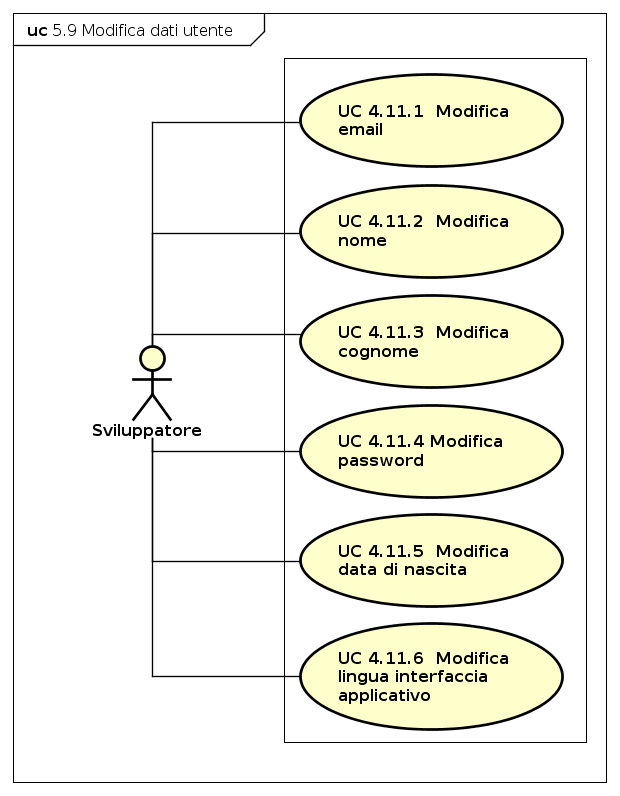
\includegraphics[width=12cm, keepaspectratio]{img/UC411.png} 
	\caption{Caso d'uso UC 4.11:  Modifica dati utente per Sviluppatore}\label{fig:411}
\end{figure}
\begin{itemize}
	\item[•]\textbf{Attori}: Sviluppatore;
	\item[•]\textbf{Descrizione}: lo sviluppatore modifica i propri dati personali, cioè tutti i dati personali inseriti in fase di registrazione;
	\item[•]\textbf{Precondizione}: lo sviluppatore visualizza la propria dashboard;
	\item[•]\textbf{Postcondizione}: lo sviluppatore ha modificato uno o più dati personali; 
	\item[•]\textbf{Flusso degli eventi}: 
	\begin{enumerate}
		\item Selezione procedura modifica dati personali;
		\item UC 4.11.1 - Modifica email; 
		\item UC 4.11.2 - Modifica nome;
		\item UC 4.11.3 - Modifica cognome;
		\item UC 4.11.4 - Modifica password;
		\item UC 4.11.5 - Modifica data di nascita;
		\item UC 4.11.6 - Modifica lingua interfaccia applicativo;
		\item Conferma modifica dati.
	\end{enumerate}
\end{itemize}
\subsubsection{UC 4.11.1 - Modifica email}
\begin{itemize}
	\item[•]\textbf{Attori}: Sviluppatore;
	\item[•]\textbf{Descrizione}: lo sviluppatore modifica la propria email;
	\item[•]\textbf{Precondizione}: lo sviluppatore sta modificando i propri dati personali;
	\item[•]\textbf{Postcondizione}: lo sviluppatore ha modificato la propria email; 
	\item[•]\textbf{Flusso degli eventi}: 
	\begin{enumerate}
		\item Selezione campo email;
		\item Modifica la stringa che rappresenta la propria email.
	\end{enumerate}
\end{itemize}
\subsubsection{UC 4.11.2 - Modifica nome}
\begin{itemize}
	\item[•]\textbf{Attori}: Sviluppatore;
	\item[•]\textbf{Descrizione}: lo sviluppatore modifica il proprio nome;
	\item[•]\textbf{Precondizione}: lo sviluppatore sta modificando i propri dati personali;
	\item[•]\textbf{Postcondizione}: lo sviluppatore ha modificato il proprio nome; 
	\item[•]\textbf{Flusso degli eventi}: 
	\begin{enumerate}
		\item Selezione campo nome;
		\item Modifica la stringa che rappresenta il nome.
	\end{enumerate}
\end{itemize}
\subsubsection{UC 4.11.3 - Modifica cognome}
\begin{itemize}
	\item[•]\textbf{Attori}: Sviluppatore;
	\item[•]\textbf{Descrizione}: lo sviluppatore modifica il proprio cognome;
	\item[•]\textbf{Precondizione}: lo sviluppatore sta modificando i propri dati personali;
	\item[•]\textbf{Postcondizione}: lo sviluppatore ha modificato il proprio cognome; 
	\item[•]\textbf{Flusso degli eventi}: 
	\begin{enumerate}
		\item Selezione campo cognome;
		\item Modifica la stringa che rappresenta il cognome.
	\end{enumerate}
\end{itemize}
\subsubsection{UC 4.11.4 - Modifica password}
\begin{figure}[H]
	\centering
	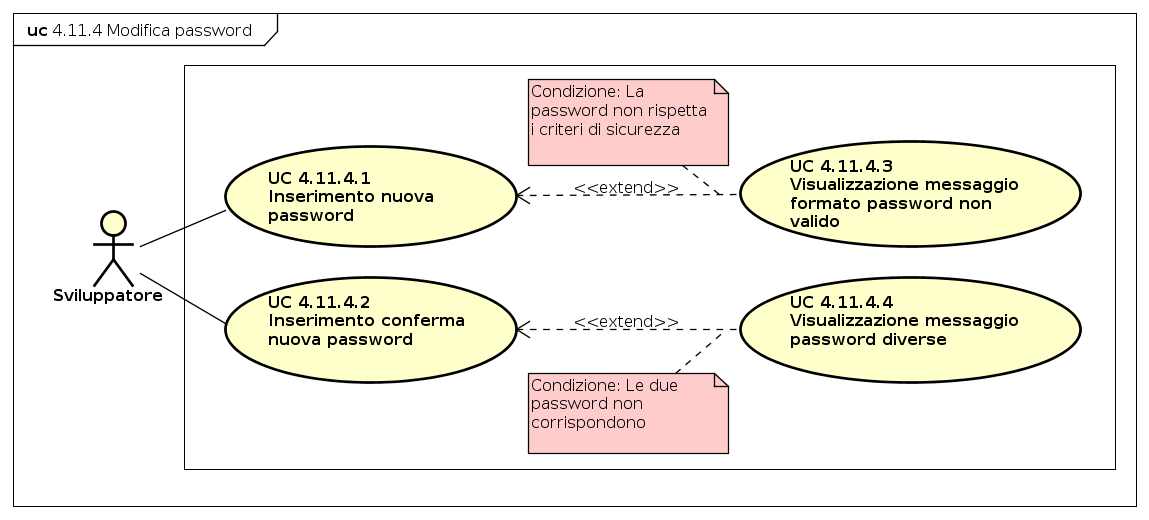
\includegraphics[width=15cm, keepaspectratio]{img/UC4114.png} 
	\caption{Caso d'uso UC 4.11.4, modifica password per Sviluppatore}\label{fig:4114}
\end{figure}
\begin{itemize}
	\item[•]\textbf{Attori}: Sviluppatore;
	\item[•]\textbf{Descrizione}: lo sviluppatore modifica il proprio cognome;
	\item[•]\textbf{Precondizione}: lo sviluppatore sta modificando i propri dati personali;
	\item[•]\textbf{Postcondizione}: lo sviluppatore ha modificato il proprio cognome; 
	\item[•]\textbf{Flusso degli eventi}: 
	\begin{enumerate}
		\item UC 4.11.4.1 - Inserimento nuova password;
		\item UC 4.11.4.2 - Inserimento conferma nuova password.
	\end{enumerate}
\end{itemize}

\subsubsection{UC 4.11.4.1 - Inserimento nuova password}
\begin{itemize}
	\item[•]\textbf{Attori}: Sviluppatore;
	\item[•]\textbf{Descrizione}: lo sviluppatore inserisce la nuova password;
	\item[•]\textbf{Precondizione}: lo sviluppatore sta modificando i propri dati personali;
	\item[•]\textbf{Postcondizione}: lo sviluppatore ha inserito il valore della nuova password; 
	\item[•]\textbf{Flusso degli eventi}: 
	\begin{enumerate}
		\item Selezione campo dati relativo alla nuova password;
		\item Inserimento stringa rappresentante la password.
	\end{enumerate}
	\item[•]\textbf{Estensioni}:
	\begin{enumerate}
		\item UC 4.11.4.3 - Visualizzazione messaggio formato password non valido.
	\end{enumerate}
\end{itemize}

\subsubsection{UC 4.11.4.2 - Inserimento conferma nuova password}
\begin{itemize}
	\item[•]\textbf{Attori}: Sviluppatore;
	\item[•]\textbf{Descrizione}: lo sviluppatore inserisce conferma la nuova password, reinserendola nell'apposito campo;
	\item[•]\textbf{Precondizione}: lo sviluppatore sta modificando i propri dati personali;
	\item[•]\textbf{Postcondizione}: lo sviluppatore ha inserito il valore del campo conferma nuova password; 
	\item[•]\textbf{Flusso degli eventi}: 
	\begin{enumerate}
		\item Selezione campo dati relativo alla conferma nuova password;
		\item Inserimento stringa rappresentante la password.
	\end{enumerate}
	\item[•]\textbf{Estensioni}:
	\begin{enumerate}
		\item UC 4.11.4.4 - Visualizzazione messaggio password diverse.
	\end{enumerate}
\end{itemize}

\subsubsection{UC 4.11.4.3 - Visualizzazione messaggio formato password non valido}
\begin{itemize}
	\item[•]\textbf{Attori}: Sviluppatore;
	\item[•]\textbf{Descrizione}: lo sviluppatore ha inserito una password con un formato non valido;
	\item[•]\textbf{Precondizione}: lo sviluppatore sta modificando i propri dati personali;
	\item[•]\textbf{Postcondizione}: lo sviluppatore visualizza un messaggio di errore relativo all'inserimento di una password che non rispetta un formato valido; 
	\item[•]\textbf{Flusso degli eventi}: lo sviluppatore ha inserito una password che non rispetta i criteri accettati dal sistema, pertanto riceve un messaggio che indica la presenza di un formato non adatto.
\end{itemize}

\subsubsection{UC 4.11.4.4 - Visualizzazione messaggio password diverse}
\begin{itemize}
	\item[•]\textbf{Attori}: Sviluppatore;
	\item[•]\textbf{Descrizione}: lo sviluppatore ha inserito un valore di conferma password che non corrisponde al valore della nuova password inserita precedentemente, pertanto visualizza un messaggio che indica che le due password non corrispondono;
	\item[•]\textbf{Precondizione}: lo sviluppatore ha inserito il valore del campo conferma nuova password;
	\item[•]\textbf{Postcondizione}: lo sviluppatore visualizza un messaggio di errore relativo all'inserimento di una password che non combacia con quella inserita nel campo nuova password; 
	\item[•]\textbf{Flusso degli eventi}: lo sviluppatore ha inserito una password che non combacia con quella inserita nel campo nuova password, pertanto riceve un messaggio che indica la presenza di tale difformità.
\end{itemize}

\subsubsection{UC 4.11.5 - Modifica data di nascita}
\begin{itemize}
	\item[•]\textbf{Attori}: Sviluppatore;
	\item[•]\textbf{Descrizione}: lo sviluppatore modifica il proprio cognome;
	\item[•]\textbf{Precondizione}: lo sviluppatore sta modificando i propri dati personali;
	\item[•]\textbf{Postcondizione}: lo sviluppatore ha modificato il proprio cognome; 
	\item[•]\textbf{Flusso degli eventi}: 
	\begin{enumerate}
		\item Selezione campo data di nascita;
		\item Modifica la stringa che rappresenta la data di nascita, inserendo il valore corretto.
	\end{enumerate}
\end{itemize}
\subsubsection{UC 4.11.6 - Modifica lingua interfaccia applicativo}
\begin{itemize}
	\item[•]\textbf{Attori}: Sviluppatore;
	\item[•]\textbf{Descrizione}: lo sviluppatore modifica la lingua dell'applicativo;
	\item[•]\textbf{Precondizione}: lo sviluppatore sta modificando i propri dati personali;
	\item[•]\textbf{Postcondizione}: lo sviluppatore ha modificato la lingua dell'applicativo; 
	\item[•]\textbf{Flusso degli eventi}: 
	\begin{enumerate}
		\item Selezione campo dati lingua applicativo;
		\item Selezione da un elenco predefinito la lingua dell'applicativo desiderata.
	\end{enumerate}
\end{itemize}

%\subsubsection{UC 4.11.7 - Conferma modifica dati}
%\begin{itemize}
%	\item[•]\textbf{Attori}: Sviluppatore;
%	\item[•]\textbf{Descrizione}: lo sviluppatore conferma la modifica dei dati inseriti;
%	\item[•]\textbf{Precondizione}: lo sviluppatore ha modificato i propri dati;
%	\item[•]\textbf{Postcondizione}: lo sviluppatore conferma la modifica e i dati vengono registrati nel sistema; 
%	\item[•]\textbf{Flusso degli eventi}: lo sviluppatore seleziona l'opzione di conferma di modifica dati.
%\end{itemize}

\subsubsection{UC 4.12 - Logout}
\begin{itemize}
	\item[•]\textbf{Attori}: Sviluppatore;
	\item[•]\textbf{Descrizione}: lo sviluppatore effettua il logout dal sistema e viene reindirizzato alla pagina di login;
	\item[•]\textbf{Precondizione}: lo sviluppatore si è autenticato;
	\item[•]\textbf{Postcondizione}: lo sviluppatore ha chiuso la sessione e viene reindirizzato alla pagina di autenticazione; 
	\item[•]\textbf{Flusso degli eventi}: lo sviluppatore seleziona il collegamento al logout e termina la sessione.
\end{itemize}